\section{Preliminaries}
\label{sec:preliminaries}

In this section, we introduce common definitions in graph theory and formal language theory which are used in this paper.
Also, we provide a brief description of CFPQ problems.

\subsection{Basic Definitions of Graph Theory}

In this paper, we use a labeled directed graph as a data model and define it as follows.
\begin{definition} \emph{Labeled directed graph} is a tuple $D = (V, E, \Sigma)$, where
\begin{itemize}
    \item $V$ is a finite set of vertices. For simplicity, we assume that the vertices are natural numbers ranging from $0$ to $|V|-1$,
    \item $E \subseteq V \times \Sigma \times V$ is a set of labeled edges,
    \item $\Sigma$ is a set of edge labels.
\end{itemize} 
\end{definition}
%~\cite{Angles2018ThePG}

An example of the labeled directed graph $D_1$ is presented in Figure~\ref{fig:example_input_graph}. Here the set of labels $\Sigma = \{a, b\}$.

\begin{figure}[h]
	\[
	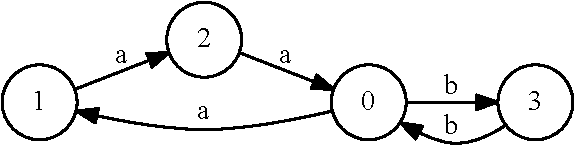
\includegraphics[width=5cm]{pictures/example_graph.pdf}
	\]
	\caption{The input graph $D_1$}
	\label{fig:example_input_graph}
\end{figure}

\begin{definition}
The \emph{path} $\pi$ in the graph $D=(V, E, \Sigma)$ is a finite sequence of labeled edges $(e_1, ..., e_{n})$, where $\forall i, 1 \leq j \leq n: e_i=(v_{i-1},l_i, v_i) \in E$.
\end{definition}

\begin{definition}
	The \emph{word} $l(\pi) \in \Sigma^*$ in the graph $D=(V, E, \Sigma)$ is the unique word $l_1 ... l_n$, obtained by concatenating the labels of the edges along the	path $\pi = (e_1 = (v_0, l_1, v_1), \ldots, e_n = (v_{n-1}, l_n, v_n))$ in the graph $D$.
\end{definition}


\subsection{Basic Definitions of Formal Languages}
We use context-free grammars as path constraints, thus in this subsection, we define context-free languages and grammars.

\begin{definition}A \emph{context-free grammar} $G$ is a tuple $(N, \Sigma, P, S)$, where
\begin{itemize}
    \item $N$ is a finite set of nonterminals
    \item $\Sigma$ is a finite set of terminals, $N \cap \Sigma = \varnothing$
    \item $P$ is a finite set of productions of the form $A \to \alpha$, where $A \in N,\ \alpha \in (N \cup \Sigma)^*$
    \item $S \in N$ is the start nonterminal
\end{itemize} 
\end{definition}

We use the conventional notation $A \xLongrightarrow[G]{*} w$ to denote, that a
string $w \in \Sigma^*$ can be derived from a non-terminal $A$ by some sequence of production rule applications from $P$ in grammar $G$.

\begin{definition} A \emph{context-free language} is a language generated by a context-free grammar $G=(N, \Sigma, P, S)$:
\begin{align*}
    L(G) &= \{w \in \Sigma^* \mid S \xLongrightarrow[G]{*} w \}.
\end{align*}
\end{definition}

\begin{definition} A context-free grammar $G = (N, \Sigma, P, S)$ is in \emph{weak Chomsky normal form} (WCNF) if every production in $P$ has one of the following forms:
    \begin{itemize}
        \item $A \rightarrow BC$, where $A, B, C \in N$
        \item  $A \rightarrow a$, where $A \in N, a \in \Sigma$
        \item $A \rightarrow \varepsilon$, where $A \in N$
    \end{itemize}
\end{definition}

Note that weak Chomsky normal form differs from Chomsky normal form in the following:
\begin{itemize}
    \item $\varepsilon$ can be derived from any non-terminal;
    \item $S$ can occur on the right-hand side of productions.
\end{itemize}

The matrix-based CFPQ algorithms process grammars only in weak Chomsky normal form, but every context-free grammar can be transformed into the equivalent grammar in Chomsky normal form~\cite{chomsky} and, therefore, it can be transformed into the weak Chomsky normal form.

Consider the context-free grammar $G_1=(\{S\},\{a, b\}, P, S)$, where $P$ contains two rules:
$S \rightarrow a \ S \ b; \ \ \ 
S \rightarrow a \ b
$.

This grammar generates the context-free language: $$L(G_1) = \{a^nb^n, n \in \mathbb{N}\}.$$
The following production rules of the grammar $G_1^{\text{wcnf}}$ is a result of the transformation of $G_1$ to weak Chomsky normal form:
\begin{align*}
S& \to A \ B   & S_1& \to S \ B   & B& \to b  \\
S& \to A \ S_1 & A& \to a &&  \\
\end{align*}


\subsection{Context-Free Path Querying}

\begin{definition}
Let $D = (V, E, \Sigma)$ be a labeled graph, $G = (N, \Sigma, P, S)$ be a context free grammar. Then a \emph{context-free relation} with grammar $G$ on the labeled graph $D$ is the relation $R_{G, D} \subseteq V \times V$:
\begin{equation*} \label{eq1}
\begin{split}
R_{G, D} = \{ &(v_0, v_n) \in V \times V  \mid \\ &\ \exists \pi = (e_1 = (v_0, l_1, v_1), \ldots, e_n = (v_{n-1}, l_n, v_n)) \in \pi(D): \\
      &\ l(\pi) \in L(G) \}.
\end{split}
\end{equation*}
\end{definition}

For example, the vertex pair $(0,0) \in R_{G_1, D_1}$, since there is a path in the labeled graph $D_1$ presented in Figure~\ref{fig:example_input_graph} from the vertex $0$ to the vertex $0$, whose labeling forms a word $$w = aaaaaabbbbbb = a^6b^6 \in L(G_1).$$

Finally, we can define context-free path querying problems.
\begin{definition}
    \emph{Context-free path querying problem with relational query semantics} is the problem of finding context-free relation $R_{G, D}$ for a given directed labeled graph $D$ and a context-free grammar $G$.
\end{definition}

In other words, the result of context-free path query evaluation is a set of vertex pairs such that there is a path between them that forms a word from the language generated by the given context-free grammar.

Using this definition, we can also define context-free path querying problems with single-path and all-path query semantics.

\begin{definition}
	\emph{Context-free path querying problem with single-path query semantics} for a given directed labeled graph $D$ and a context-free grammar $G$ is the problem of finding context-free relation $R_{G, D}$ and finding for each vertex pair $(v_0, v_n) \in R_{G, D}$ one example of a path $\pi$ between these vertices such that $l(\pi) \in L(G)$.
\end{definition}

\begin{definition}
	\emph{Context-free path querying problem with all-path query semantics} for a given directed labeled graph $D$ and a context-free grammar $G$ is the problem of finding context-free relation $R_{G, D}$ and finding for each vertex pair $(v_0, v_n) \in R_{G, D}$ all paths $\pi$ between these vertices such that $l(\pi) \in L(G)$.
\end{definition}
